\textit{Out-going commands} are commands in a user application (namely in an application which sends commands to a service provider) and \textit{out-going reports} are reports in a provider application (namely in an application which sends reports to a service user).

Out-going commands and out-going reports are treated together because their management is performed in the same way and is based on the following components:

\begin{fw_description}
\item[OutComponent]\hfill\\ 
This component models the generic behaviour of an out-going command or report. Concrete commands or report generated by an application are defined as extensions of the base OutComponent component. 
\item[OutFactory]\hfill\\ 
This is a component factory (in the sense of section \ref{sec:CmpInst}) which provides unconfigured instances of OutComponents to encapsulate out-going commands or reports.
\item[OutLoader]\hfill\\ 
After an application has configured an OutComponent representing an out-going command or report, it loads it into the OutLoader. This component is responsible for selecting the appropriate OutManager to process the out-going command or report. 
\item[OutManager]\hfill\\ 
This component is responsible for controlling an out-going command or report until the OutComponent which encapsulates it is serialized to the OutStream and sent to its destination as a packet.
\item[OutStream]\hfill\\ 
This component models the interface through which out-going commands and reports are sent to their destination.
\item[OutRegistry]\hfill\\ 
This component acts as a registry for pending OutComponents. It provides information about the state of the OutComponent to other parts of the host applications. 
\end{fw_description}

Note that the OutFactory, OutLoader, and OutRegistry components are singletons and it is therefore assumed that only one instance of each exists in an application. It is also assumed that there is one (and only one) OutStream for each destination to which commands may be sent (see usage constraints at the end of section \ref{sec:OutStream}).

\begin{figure}[h]
 \centering
 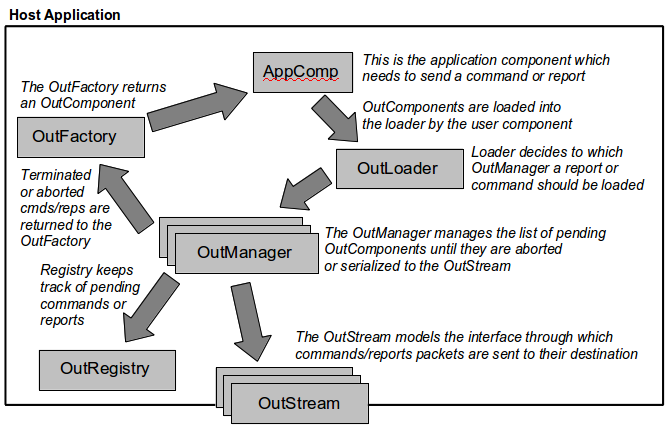
\includegraphics[scale=0.50,keepaspectratio=true]{OutGoingCmdAndRep.png}
 \caption{Management of Out-Going Commands and Reports}
 \label{fig:OutGoingCmdAndRep}
\end{figure}

The lifecycle of an out-going report or command is shown in figure \ref{fig:OutGoingCmdAndRep} using and informal notation and can be summarized as follows:
\begin{fw_enumerate}
\item When the host application decides that it must issue a command or a report, it asks the OutFactory for an unconfigured OutComponent instance to encapsulate the out-going command or report.
\item The application configures the OutComponent and then loads it in the OutLoader.
\item The OutLoader selects an OutManager and loads the OutComponent into it. The selection of the OutManager will often be based on the urgency with which the command or report must be issued (e.g. each OutManager component is characterized by a certain priority level). 
\item\label{lst:OutComponentProcessing} The OutManager component processes the out-going command or report. If the command or report is disabled, it is aborted and the component which encapsulated it is returned to its factory (where it is either destroyed or is reused). If instead the command or report is enabled, it remains pending in the OutManager until its ready check indicates that the conditions are in place for it to be issued. 
\item The report or command is issued by serializing its OutComponent to a packet which is then handed over to the OutStream. The OutStream is responsible for sending the packet to its destination. 
\item After the OutComponent has been serialized and sent to its destination, the OutManager evaluares the outcome of its Repeat Check. If this is equal to "repeat", the content of the OutComponent is updated and the OutComponent is then processed again as per point \ref{lst:OutComponentProcessing} above. If instead the repeat check had returned "no repeat", processing of the OutComponent terminates and the OutComponent is returned to its factory.
\end{fw_enumerate}


